\chapter{Lec 20 - Transformers II}

\section{RNNs vs. Transformers}
\textbf{Long-term dependencies:}
\begin{itemize}
    \item RNNs have problems in dealing with long-term dependencies between words that are spread far apart in a long sentence;

    \item Transformers do not have the above problem, as long as the long-term dependencies are in the range of the maximum allowed input length;
\end{itemize}
\textbf{Parallel computation:}
\begin{itemize}
    \item RNNs process the input sequence sequentially one token at a time: before starting the computation for time step $t$, the computation for time step $t-1$ should be completed; training and inference are slowed down;

    \item Transformers can process in parallel all the tokens in the input sequence (as well as all sequences in a batch) exploiting matrix multiplication (very efficient in GPUs);
\end{itemize}
\textbf{Context fragmentation:}
\begin{itemize}
    \item Attention can only deal with fixed-length sequences, so long sequences should be split into a certain number of segments (chunks) before being fed into a Transformer;

    \item RNNs do not have the above problem;
\end{itemize}
\textbf{Out-of-distribution generalization:}
\begin{itemize}
    \item Transformers are not able to implement recurrent rules (if they exist in data), so in principle they do not generalize well to sequences longer than the training ones;

    \item RNNs in principle can learn recurrent rules (if they exist in data);
\end{itemize}
Attention in Transformers scales quadratically with the length of the input sequence. Let $D$ be the hidden dimension of the transformer (size embeddings times \#heads). Let $T$ be the length of the input sequence.
\begin{center}
    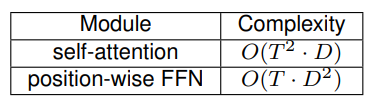
\includegraphics[]{images/attention-complexity.png}
\end{center}
Then, when the input sequences are short, the hidden dimension $D$ dominates the complexity of self-attention and position-wise FFN. The bottleneck of Transformer thus lies in FFN. However, as the input sequences grow longer, the sequence length $T$ gradually dominates the complexity of these modules, in which case self-attention becomes the bottleneck of Transformer.\newline\newline
Furthermore, self-attention does no assume any structural bias over inputs. Even the order information is also needed to be learned from training data. Therefore, Transformer (w/o pre-training) is usually easy to overfit on small or moderate-size data.

\section{X-formers}
\textbf{X-formers} improve the vanilla Transformer from different perspectives:
\begin{itemize}
    \item \textbf{Model Efficiency:} In the standard self-attention mechanism, every token needs to attend to all other tokens. However, it is observed that for the trained Transformers the learned attention matrix $\textbf{A}$ is often very sparse across most data points.  Therefore, it is possible to reduce computation complexity by incorporating structural bias to limit the number of query-key pairs that each query attends to.
    \begin{center}
        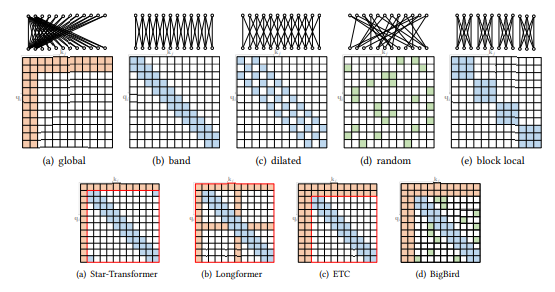
\includegraphics[]{images/x-formrs.png}
    \end{center}
    Another effective way of dealing with long sequences is to use \textbf{divide-and-conquer} strategy, i.e., to decompose an input sequence into finer segments that can be efficiently processed by Transformer or Transformer modules.

    \item \textbf{Model Generalization:} Transformers can be pre-trained on large-scale unlabeled data.

    \item \textbf{Model Adaptation:} Transformers adapted to specific downstream tasks and applications.

\end{itemize}

\section{Model Pre-training}
Recent studies suggest that Transformer models that are pre-trained on large corpora can learn universal language representations that are beneficial for downstream tasks. The models are pre-trained using various self-supervised objectives:
\begin{itemize}
    \item  \textbf{Decoder only.}
    
    \item \textbf{Encoder only.}

    \item \textbf{Encoder-Decoder.}
\end{itemize}
After pre-training a model, one can simply fine-tune it on downstream datasets, instead of training a model from scratch.

\subsection{Language model via a Decoder}
The idea is to train a decoder to predict the next word/token in the sentence. Then, we fine-tune the resulting model to perform the learning task.

\subsubsection{Generative Pre-Trained Transformer (GPT)}
Given a corpus of unsupervised tokens $U = \{u_1,..., u_n\}$, we first train a multi-layer transformer Decoder to maximize:
\[L_1(U) = \sum_i log\,P(u_i | u_{i-k}, ..., u_{i - 1}, \Theta)\]
\begin{center}
    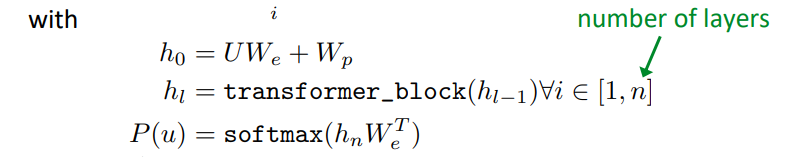
\includegraphics[scale=0.6]{images/GPT.png}
\end{center}
Then, after the pre-training phase, we add on top of the decoder a softmax linear classifier and fine-tune the whole model (decoder + linear classifier) on the main learning task.\newline\newline
The first version of GPT was a Transformer decoder with 12 layers, 768-dimensional hidden states, 3072-
dimensional feed-forward hidden layers; Byte-pair encoding with 40,000 merges; Trained on BooksCorpus: over 7000 unique books.\newline\newline
\textbf{GPT-2} is a Larger version of GPT (1.5 billion parameters) trained on more data, was shown to produce relatively convincing samples of natural language.\newline\newline
\textbf{GPT-3} is a Huge model: 175 billion parameters.

\subsection{Masked Language Model via encoder}
Decoders only take left context, while encoders are bidirectional (both left and right context), so how to train an encoder to perform Language Modeling ? We can perform \textbf{Mask Language Modeling} (MLM). Basically, we replace some fraction of words in the input with a special [MASK] token, and the self-supervised learning task is to predict these masked words.\newline\newline
For example:
\begin{itemize}
    \item original sentence: I went to the store.

    \item masked sentence: I [M] to the [M].
\end{itemize}

\subsubsection{BERT: Bidirectional Encoder Representations from Transformers}
A model based on MLM is BERT. The idea is to predict a random 15\% of (sub)word tokens. In particular, the words are \textit{masked} in 3 different ways:
\begin{itemize}
    \item Replace the input word with [MASK] 80\% of the time;

    \item Replace the input word with a random token 10\% of the time;

    \item Leave the input word unchanged 10\% of the time (but still predict it!)
\end{itemize}
\begin{center}
    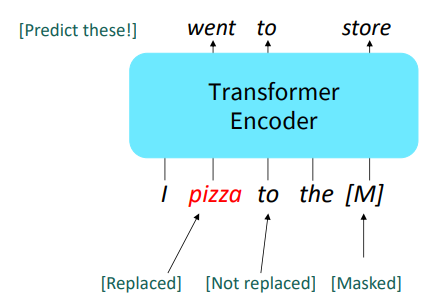
\includegraphics[scale=0.8]{images/BERT.png}
\end{center}
This is done in order to make the model able to learn strong representations of non-masked words too.\newline\newline
Two models were released:
\begin{itemize}
    \item BERT-base: 12 layers, 768-dim hidden states, 12 attention heads, 110 million params.

    \item BERT-large: 24 layers, 1024-dim hidden states, 16 attention heads, 340 million params.
\end{itemize}
Overall pre-training and fine-tuning procedures for BERT. Apart from output layers, the same architectures are used in both pre-training and fine-tuning.

\subsection{Language Model via encoder-decoder}
Encoders don’t naturally lead to effective autoregressive (1-word-at-a-time) generation methods as decoders do. The idea is to use an encoder-decoder architecture in order to make the model able to perform both natural language understanding and generation.\newline\newline
In order to do this, we can replace different-length spans from the input
with unique placeholders, and decode out the spans that were removed.

